\section{Methodology}
\ac{CUPID} aims to generate pure shift spectra by utilising the result of
parametric estimation of \ac{2DJ} data, assumed to take the functional form of
\eqref{eq:jres-fid}. In this section, a description of the method is given.

\subsection{The estimation routine}
The primary steps involved in estimating a \ac{2DJ} dataset are
\begin{enumerate}
    \item Generation of a frequency-filtered sub-\ac{FID} (Section
        \ref{subsec:jres-filtering}).
    \item Prediction of the model order, either by applying the \ac{MDL} on the
        first \ac{FID} in the direct dimension (Section
        \ref{subsec:model-order}) or by manually specifying a
        value.
    \item Generation of an initial guess using the \ac{MMEMPM} (Section
        \ref{subsec:mmempm}).
    \item Subjection of the initial guess to \ac{NLP} (Section \ref{sec:nlp}).
\end{enumerate}
Instead of estimating successive \ac{1D} \acp{FID}, as proposed by
Nuzillard and Mutzenhardt et al., \ac{2DJ} sub-\acp{FID} are estimated
holistically. By doing this, a number of benefits are realised.
Firstly, multiplet structures which heavily overlap in a
conventional \ac{1D} dataset become separated in the \ac{2DJ} dataset (assuming
that the Larmor frequencies of the relevant spins are sufficiently different).
Accurate resolution of the signal components in more crowded spectral
regions is far more likely to be successful with a full \ac{2D} estimation as a
result.
On top of this, there is an extra resolution advantage relative to the
estimation of \emph{direct} dimension \acp{FID}. Due to the presence of a spin
echo during $\tone$, signal damping effects caused by field inhomogeneities are
nullified, such that damping is dictated solely by transverse relaxation
($T_2$). During $\ttwo$ however, the influence of field inhomogeneities are not
corrected, such that damping occurs at a faster rate, characterised by $T_2^*$.
As such, multiplet structures in the indirect dimension exhibit better
resolution (assuming $\nicefrac{\fswone}{\None}$ and
$\nicefrac{\fswtwo}{\Ntwo}$ are comparable).
A further benefit comes with having access to the frequencies of each
oscillator in \emph{both} dimensions, since this allows one to group together
those which belong to the same multiplet (see Section
\ref{subsec:mp-selection}). Similar information can be obtained
by extracting slices of a tilted magnitude-mode \ac{2DJ} spectrum at
appropriate values of $F^{(2)}$, though the lineshapes of peaks suffer from the
undesirable characteristics described above. The
\ac{ZS}-\ac{2DJ}\cite{Pell2007} and
\ac{PSYCHE}-\ac{2DJ}\cite{Foroozandeh2015,Kiraly2017} experiments are also able
to generate individual multiplet structures, though with long \ac{3D} pulse
sequences, and with reduced sensitivity relative to a conventional \ac{2DJ}
experiment.

As was mentioned in Section \ref{subsec:model-order}, application of the
\ac{MDL} to a \ac{2D} \ac{FID} is not desirable, since a full \ac{SVD} would
need to be computed on the Hankel matrix $\symbf{E}_{\symbf{Y}}$.
Assuming that the spectral region being considered is not too
crowded, applying the \ac{MDL} on the first direct-dimension \ac{FID} can
return reasonable estimates of $M$ at a far smaller computational cost. For
particularly crowded regions, resorting to a manual specification of model
order by inspecting the \ac{2DJ} spectrum is the best solution currently
available.
An interesting benefit is realised when the \ac{1D} \ac{MDL} is applied.
As described above, the presence of strong coupling artefacts introduces
nuisance peaks into spectra produced by shearing and summation. Exactly the
same effect would be realised using estimation, assuming
that the relevant signals are quantified. However, since strong coupling
artefacts have direct-dimension frequencies which are identical to those of
first-order signals in the dataset, it is virtually impossible to resolve these
using the \ac{1D} \ac{MDL} approach. Therefore the \ac{MDL} is often found to
generate a model order which agrees with the number of \emph{first-order} signals,
rather than the \emph{true} number of signals in the \ac{FID}. As the
\ac{MMEMPM} generates a parameter estimate based on the first $M$ significant
components of the dataset, the more intense first-order signals are quantified,
whereas the weaker strong coupling artefacts are not included.

\subsection{The \ang{-45} signal}
\begin{figure}
    \centering
    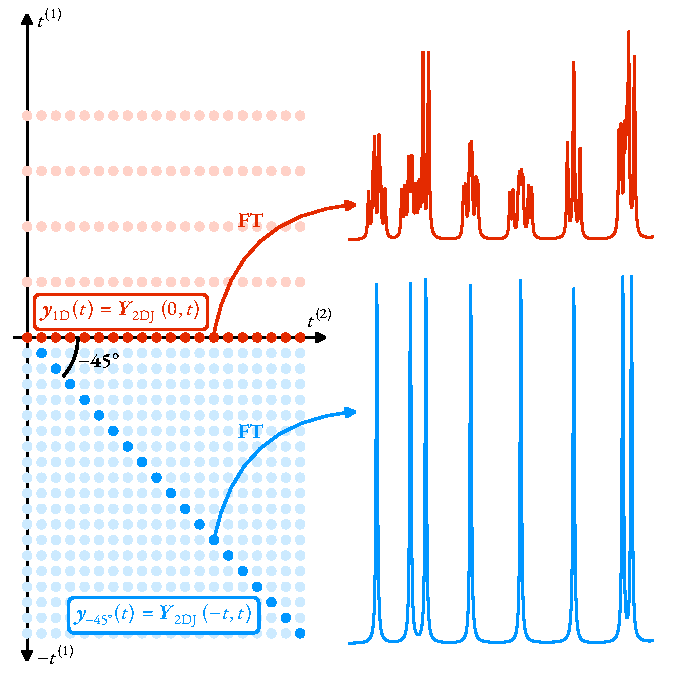
\includegraphics{neg_45_signal/neg_45_signal.pdf}
    \caption[
        An illustration of the reasoning behind the name ``\ang{-45}
        signal'' used to generate pure shift spectra.
    ]{
        An illustration of the reasoning behind the name ``\ang{-45}
        signal'', which is used to generate pure shift spectra. The pale red
        dots denote
        a typical \ac{2DJ} \ac{FID}, where
        the amount and rate of sampling in the direct dimension is greater than
        in the indirect dimension (i.e. $\None \ll \Ntwo$ and $\fswone \ll
        \fswtwo$). The bright red dots correspond to the first direct-dimension
        signal $y(0,\ttwo)$, which has the same form as
        \iac{FID} from a pulse-acquire experiment. A hypothetical signal
        generated by propagating the \ac{FID} into $-\tone$, with the same rate
        of sampling in both dimensions, is denoted with pale blue dots. Taking
        the diagonal of this signal, such that it forms a \ang{-45} angle to the
        $\ttwo$ axis, yields an \ac{FID} $\by_{\ang{-45}}$  which is
        homodecoupled. Note that there is a slight discrepancy
        between \eqref{eq:neg-45} and this description, in that the
        indirect-dimension damping factors $\bdetaone$ are neglected in the
        former case.
    }
    \label{fig:neg-45}
\end{figure}
The \ac{2DJ} estimation routine generates a parameter vector $\bth \in
\mathbb{R}^{6M}$. With
knowledge of the frequencies and damping factors in both dimensions, it is
possible to generate \iac{FID} which will produce a pure shift spectrum
directly, rather than constructing a full-echo \ac{2DJ} signal, and
subsequently shearing and summing it. The desired signal is named
the \emph{\ang{-45} signal} $\symbf{y}_{\ang{-45}} \in \mathbb{C}^{\Ntwo}$:
\begin{equation}
    y_{\ang{-45},\ntwo} =
        \sum_{m=1}^{M} a_m \exp (\iu \phi_m)
        \exp\left(\left(2 \pi \iu \left(\ftwo_m - \fone_m - \foff\right)
                - \etatwo_m
            \right) \ntwo \Dttwo
        \right),
    \label{eq:neg-45}
\end{equation}
with the reasoning behind the name provided by Figure \ref{fig:neg-45}.
The \ang{-45} signal
takes the form of a \ac{1D} \ac{FID} expected from a pulse-acquire experiment,
except that the frequency of each oscillator, which would usually be $\ftwo_m$,
is replaced with $\ftwo_m - \fone_m$, such that oscillators belonging to a
given multiplet all provide a contribution with the frequency $\omega_{0,s}$.
Assuming that the parameters associated with the \ac{2DJ}
\ac{FID} are accurately determined, a pure shift spectrum with sharp
absorption-mode lineshapes and no loss of signal can be generated by
constructing the \ang{-45} signal.


\subsection{Filtration of \ac{2DJ} data}
\label{subsec:jres-filtering}
Unlike the direct-dimension, which can often comprise sparsely distributed
peaks in the Fourier domain, the indirect dimension of \ac{2DJ} datasets tends
to be densely populated since all multiplet structures are centered at
\qty{0}{\hertz}, and rarely span beyond $\pm \qty{50}{\hertz}$. As such,
generation of frequency-filtered sub-\acp{FID} is limited to consideration of
the direct dimension.
The filtering procedure applied to \ac{2DJ} data is an extension of that
for \ac{1D} data described in Section \ref{sec:filtering}, and is
depicted in Figure \ref{fig:jres-filtering}:
\begin{enumerate}
    \item The signal $\symbf{Y}_{\text{ve}} \in \mathbb{C}^{\None \times 2 \Ntwo}$ is
    constructed, such that a virtual echo is formed from each direct-dimension
    signal. Each row of the signal $\by_{\text{ve},\none}\ \forall n^{(1)} \in
    \lbrace 0, \cdots, N^{(1)} - 1 \rbrace$ given by
    \begin{equation}
        \by_{\text{ve},\none} =
            \begin{bmatrix}
                \Re\left(y_{n^{(1)}, 0}^{\vphantom{*}}\right) &
                y_{n^{(1)}, 1}^{\vphantom{*}} &
                \cdots &
                y_{n^{(1)}, \Ntwo - 1}^{\vphantom{*}} &
                0 &
                y_{n^{(1)}, \Ntwo - 1}^* &
                \cdots &
                y_{n^{(1)}, 1}^*
            \end{bmatrix}.
    \end{equation}
    \item $\symbf{Y}_{\text{ve}}$ is subjected to \ac{FT} along the direct
        dimension to produce the spectrum  $\symbf{S}_{\text{ve}}$ (panel a of
        Figure \ref{fig:jres-filtering}). This has an imaginary component of
        zero.
    \item A super-Gaussian $\symbf{G} \in \mathbb{R}^{\None \times 2 \Ntwo}$ is
        constructed (panel b):
        \begin{equation}
            \symbf{G} = \symbf{1} \otimes \symbf{g}^{(2)},
        \end{equation}
        where $\symbf{1} \in \mathbb{R}^{\None}$ is a vector of ones, and
        $\symbf{g}^{(2)} \in \mathbb{R}^{2\Ntwo}$ is a super-Gaussian vector
        given by \eqref{eq:super-Gaussian-onedim}.
    \item A matrix of additive noise is generated by extracting the variance
        $\sigma^2$ of a direct-dimension strip of $\symbf{S}_{\text{ve}}$ which
        is devoid of peaks, and generating an array $\symbf{W}_{\sigma^2} \in
        \mathbb{R}^{\None \times 2 \Ntwo}$ with values independently sampled
        from a normal distribution with mean $0$ and variance  $\sigma^2$.
    \item The spectrum is filtered (panel d):
        \begin{equation}
            \widetilde{\symbf{S}}_{\text{ve}} = \symbf{S}_{\text{ve}} \odot
            \symbf{G} + \symbf{W}_{\sigma^2} \odot (\symbf{1} - \symbf{G}).
        \end{equation}
    \item $\widetilde{\symbf{S}}_{\text{ve}}$ is subjected to \ac{IFT} and is
        sliced in half in the direct dimension, yeilding the final filtered
        signal $\widetilde{\symbf{Y}}$.
\end{enumerate}

\begin{figure}
    \centering
    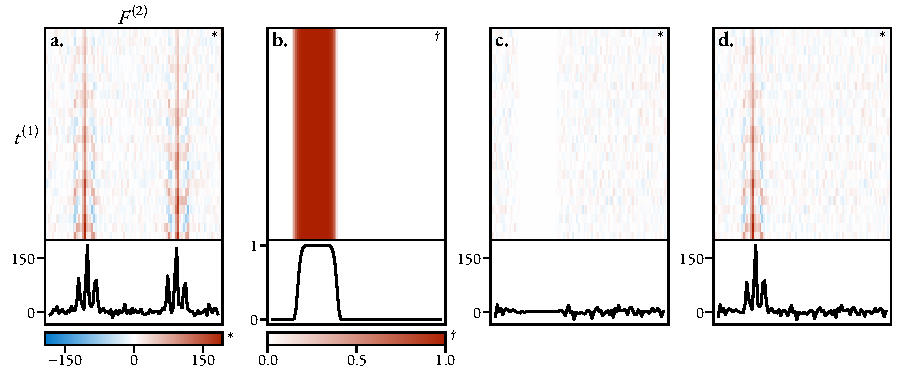
\includegraphics{jres_filtering/jres_filtering.pdf}
    \caption[
        An illustration of the filtering procedure for \ac{2DJ} data.
    ]
    {
        An illustration of the filtering procedure for \ac{2DJ} data.
        For each panel is a heat-map of the full \ac{2D} signal, as well as a
        plot underneath of the first slice of the signal in the direct
        dimension.
        \textbf{a.} The spectrum $\symbf{S}_{\text{ve}}$,
        \textbf{b.} Super-Gaussian filter $\symbf{G}$,
        \textbf{c.} Additive noise, attenuated by the super-Gaussian, $\symbf{W}_{\sigma^2} \odot (\symbf{1} - \symbf{G})$,
        \textbf{d.} Filtered spectrum $\widetilde{\symbf{S}}_{\text{ve}}$
        Panels \textbf{a.}--\textbf{d.} are analogous to panels \textbf{b.}--
        \textbf{e.} in Figure \ref{fig:filtering} for the \ac{1D} case.
    }
    \label{fig:jres-filtering}
\end{figure}


\subsection{Multiplet Prediction}
\label{subsec:mp-selection}
\ac{CUPID}'s ability to group oscillators present in a parameter set into
multiplet structures relies knowledge of both thw indirect- and
direct-dimension frequencies of each oscillator. As has already been
established, for oscillators which are associated with the same multiplet
grouping $G_s$, the quantities $\ftwo_{m_1} - \fone_{m_1}$ and $\ftwo_{m_2} -
\fone_{m_2}$ should be equal ($\omega_{0,s}$) for any pairing  $m_1, m_2 \in
G_s$. An assessment of whether two oscillators belong to the same multiplet can
therefore be made using the following criterion:
\begin{equation}
    \left \lvert
        \left( \ftwo_{m_1} - \fone_{m_1} \right) -
        \left( \ftwo_{m_2} - \fone_{m_2} \right)
    \right \rvert < \epsilon.
\end{equation}
$\epsilon \in \mathbb{R}_{>0}$ is a suitable threshold to account for error in
the estimation result. A lower bound on the threshold is the separation between
adjacent points in the better resolved dimension of the spectrum, i.e.
$\epsilon = \min\left(\nicefrac{\fswone}{\None},
\nicefrac{\fswtwo}{\Ntwo}\right)$.  However, limitations in resolution due to
signal damping and field inhomogeneities can mean that $\epsilon$ has to be
increased beyond this for reasonable multiplet assignments to be achieved.
Listing \ref{lst:mp-assign} provides a \Python routine that can be used for multiplet
prediction.

% Spurious oscillators:
% \begin{itemize}
%     \item Very broad, with $\fone \approx \qty{0}{\hertz}$. Caused in cases where very intense signal i.e. from solvent/residual water has a tail which ``breaks into'' the region of interest.
%     \item Low intensity, random indirect frequency: overfit: probably fitting a
%         noise component
%     \item Around region boundary: likely due to artefacts induced by filtering
% \end{itemize}
% The ability to predict multiplet groupings can also assist in scenarios where
% the estimation result contains some oscillators with a spurious nature,
% typically due to overfitting. These typically possess either a very large
% damping factor or low amplitude, and are not associated with discernible peaks
% in the spectrum. Part of the reason that the variance of phases is included in
% the fidelity for \ac{NLP} is to try and purge these oscillators, however this
% method is not infallible, and undesired oscillators can end up in the final
% result. An appreciable number of these can be removed in an automated fashion
% by noting that there should not be any oscillators in the estimation result of
% a 2DJ dataset which satisfy both of the following:
% \begin{enumerate}
%     \item The oscillator is not grouped with any other oscillator as part of
%         the multiplet assignment.
%     \item The magnitude of the indirect dimension frequency of the oscillator
%         is appreciably greater than \qty{0}{\hertz}.
% \end{enumerate}
% These criteria are borne out of the fact that it should not be possible to have
% oscillators in a 2DJ dataset which are not part of a multiplet structure,
% unless such oscillators are singlets. As no scalar couplings contribute, these
% singlets should have an indirect dimension frequency of \qty{0}{\hertz}.
